%------------------------------------------------------------------------------
%
%------------------------------------------------------------------------------

Cowhub is built using state of the art image recognition and cloud computing technology. However, the key of this project is to provide farmer with an intuitive and easy to use cattle management and identification solution. Hence the conceptualisation of our front ends was human centered.

%------------------------------------------------------------------------------

\begin{subsection}{Persona}
  We designed the following persona to portrait the potential users of Cowhub. Doing so allowed us to extract the demographic characteristics, the needs, the values and lifestyle of farmers.
  \begin{figure}[H]
  	\centering
    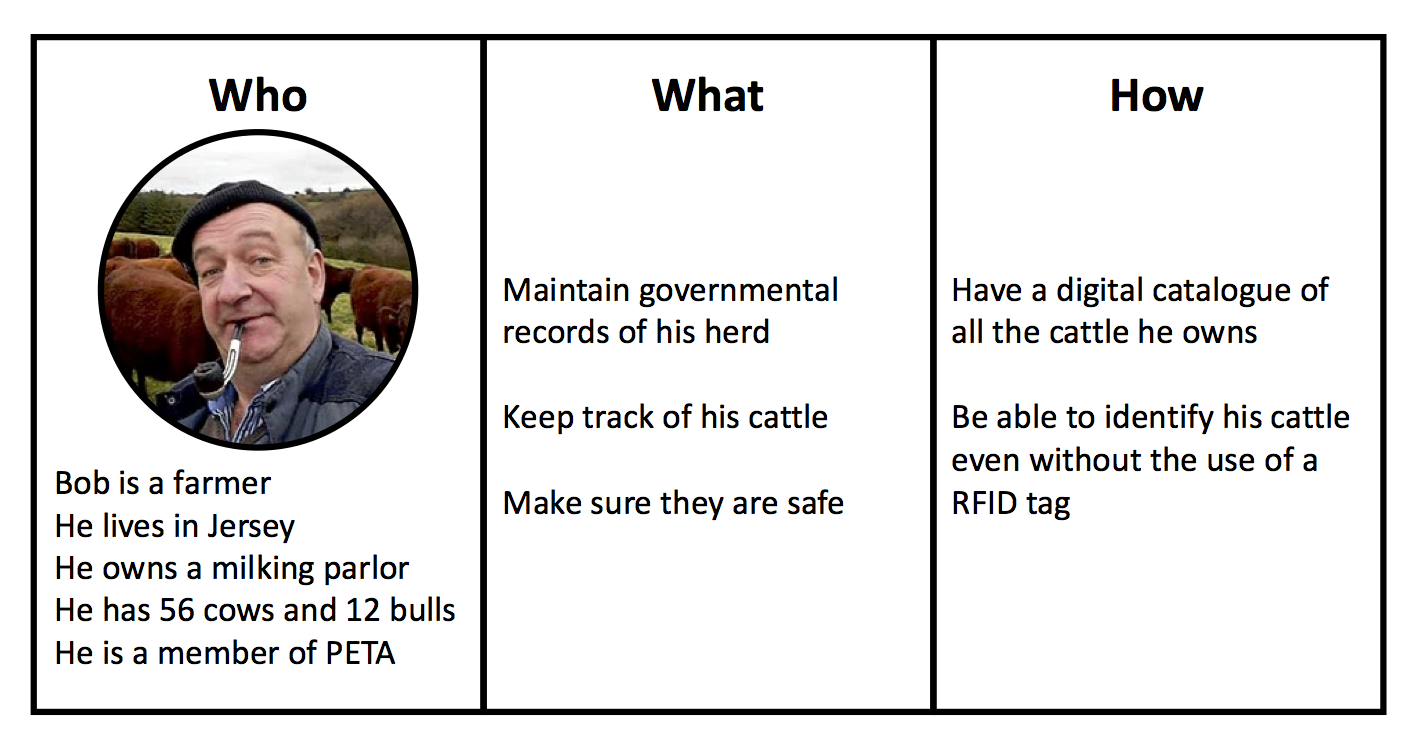
\includegraphics[width=1\textwidth]{images/persona.png}
  	\caption[Persona]{Persona - Bob the farmer}
  \end{figure}
\end{subsection}

%------------------------------------------------------------------------------

\begin{subsection}{User Stories}
  From the persona described above we derived the main user stories our app must implement:
  \begin{enumerate}
    \item As as a farmer, I want to have a portable cattle registration tool, so I can easily maintain my governmental records.
    \item As a farmer, I want to have a digital catalogue of my herd, so I can manage my cattle.
    \item As a farmer, I want to have an cattle identification tool, so I can recognize a lost cow by simply taking its picture.
  \end{enumerate}
\end{subsection}

%------------------------------------------------------------------------------

\begin{subsection}{Service blueprint}
  Based on the user stories we then conceived our user journeys, see Figures \ref{fig:register-cattle-journey} and \ref{fig:identify-cattle-journey}.
  \begin{sidewaysfigure}
    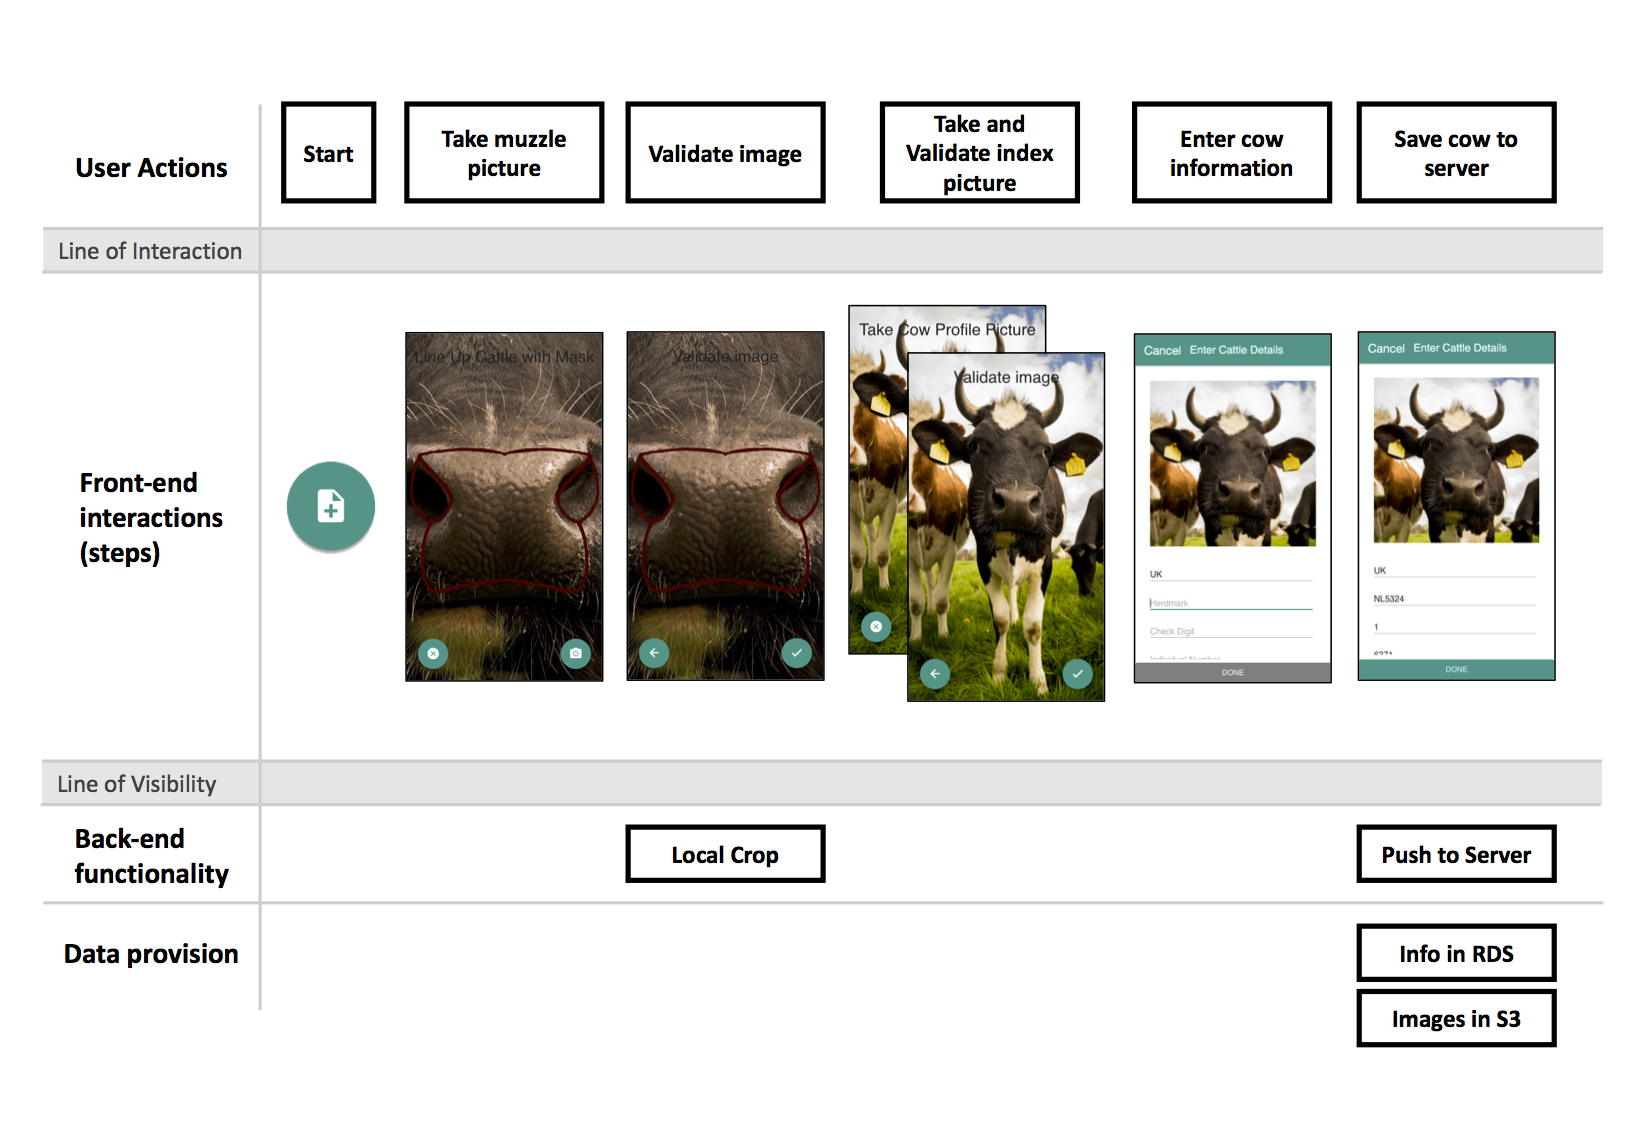
\includegraphics[width=\textwidth]{images/register-cattle-journey.png}
    \caption{Cattle Registration Journey}
    \label{fig:register-cattle-journey}
  \end{sidewaysfigure}
  \begin{sidewaysfigure}
    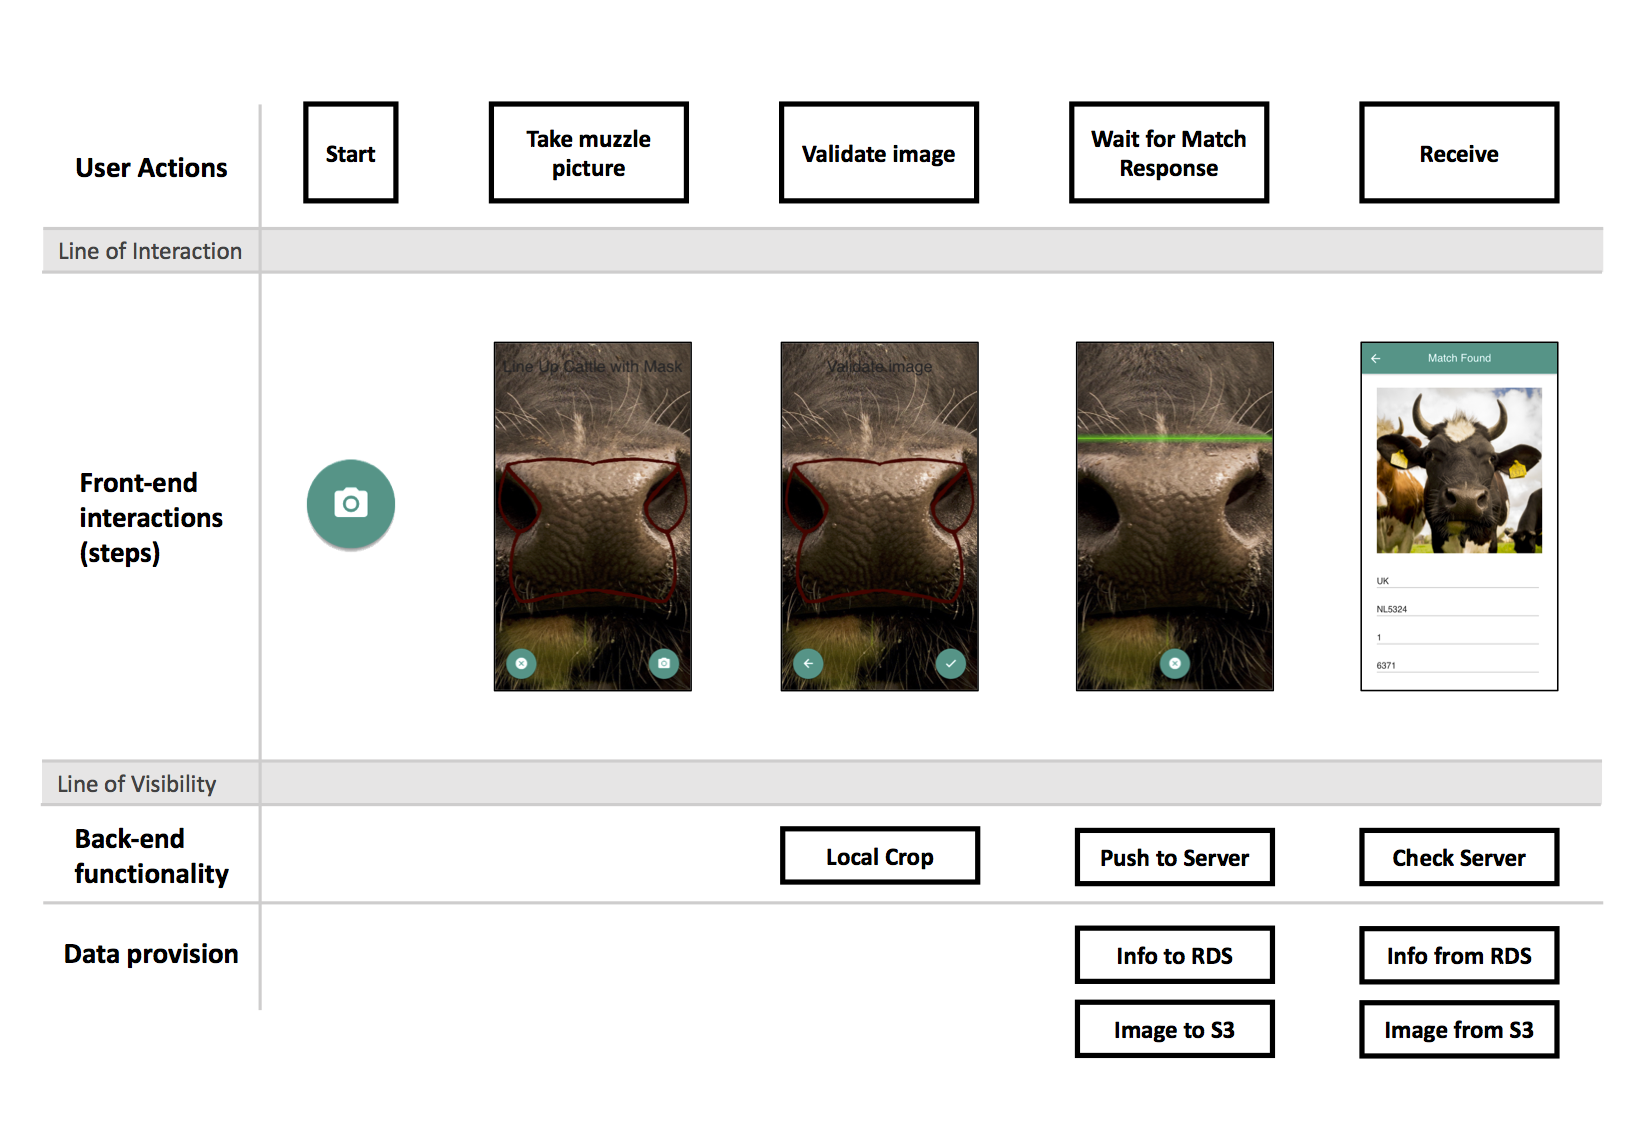
\includegraphics[width=\textwidth]{images/identify-cattle-journey.png}
    \caption{Cattle Identification Journey}
    \label{fig:identify-cattle-journey}
  \end{sidewaysfigure}
\end{subsection}

%------------------------------------------------------------------------------

\begin{subsection}{User Feedback}
  Most importantly we want to have feedback from actual farmers who will potentially use our tool. Therefore we traveled to Jersey and tested the platform on the field. We also used this opportunity to interview cattle cartakers and breeders to gain some insight that might lead to further improve the performance of our recognition algorithm. Here is an extract:
\end{subsection}
